\chapter{Framework Implementation}
\label{sec:impl}
\section{Architecture Decision}
\subsection{Available Alternatives}
Based on the requirements outlined in section \ref{sec:reqanalysis}, which have been gathered and derived in various in-person meetings with the stakeholding therapists, multiple technologies for implementing the system seem feasible. The alternatives considered at the beginning of this project are outlined as follows.

\subsubsection{Fully featured Web Application}
\label{sec:alt:fully-featured-web-app}
One technological possibility would be to implement the core system framework as a fully featured Web Application. All requirements would be implemented using web technologies. Most notably, data ingestion, preprocessing, classification, and monitoring would have to be accomplished entirely in the context of a web browser. The system would be self-sufficient in this configuration, without reliance on any external systems, though an external server component for sending the monitoring information is conceivable (see requirement \ref{sec:req:monitorability}).

This configuration is very favorable in terms of deployment and extensibility, as every component is consistently written in Javascript, the standardized programming language of the web. Likewise, as functionality is not distributed over multiple systems, the deployment of the systems only requires a web browser\footnote{The installation of relevant hardware device drivers on the target device is also required for the system to function, but as the same is true for all other alternatives, this is not considered under the ease of deployment aspect.}.

However, for this configuration to be feasible, it is required that the domain virtualization device contains an API to the Web Browser. Also, the Javascript programming language is sometimes critizied for its relatively poor performance when compared to programming languages with compilers capable of producing native code. This is owed in large parts to the dynamically typed and interpreted nature of the language. Some benchmarks show that Javascript is up to ten times slower in terms of runtime performance compared to C++ when running computationally expensive tasks \cite{BenchmarksGame}. The question of whether Javascript is performant enough to tackle the task at hand has to be clarified before this alternative can be considered feasible.
\subsubsection{Web Application with local server component}
\label{sec:alt:thin-web-app}
The two main disadvantages of the fully featured Web Application, the need for a Web API of the virtualization device and the performance considerations, could be mitigated by moving the computationally expensive logic in a locally running server component, and interfacing the two components by using an asynchronous communication specifications such as WebSockets or XmlHttpRequest. As the code running in the server component is running with Operating System permissions, it could directly interface with the hardware device. Additionally, all logic concerned with working with the virtualization device data could be implemented in native code, resulting in high performance.

This approach in turn poses the disadvantage that a lot of additional complexity is introduced into the system. The system would no longer be implemented in a single programming language. Additionally, the system would no longer be easy to deploy, as compiled binary packages would have to be provided and thoroughly tested for each desired target Operating System.
\subsubsection{Web Application with remote server component (backend)}
\label{sec:alt:thin-remote-web-app}
Following up on the design outlined in section \ref{sec:alt:thin-web-app}, the system could also be designed with a remote server component instead of a locally running server. This would have the advantage of all device data being available
at one centralized location, where very elaborate analytics could be performed. As all alternatives outlined in this section will eventually require a backend component for accumulating monitoring information for the therapist to view and inspect, this approach initially seems to reduce complexity.

However, the virtualized domain data would again have to be ingested by the Web Application, in a similar fashion to the alternative outlined in \ref{sec:alt:fully-featured-web-app}, as no local application is available to handle the connection to the hardware device. Furthermore, all virtualization device data would have to be sent over the network connection of the end device, potentially resulting in high latency, and possibly full system outage if the end device fails to establish an internet connection.
\subsubsection{Desktop Application}
\label{sec:alt:desktop-app}
Finally, the system could be designed without relying on Web technologies altogether, and be instead implemented as a traditional Desktop Application.

\begin{table}[h]\footnotesize
\caption{Comparison of implementation alternatives based on estimated requirement fulfillment}
\label{alt:table-requirement-comparison}
\renewcommand{\arraystretch}{1.3}
\begin{tabular}{l|cccccc}
    &
    \rot{Functional Reqs.} &
    \rot{Modularization} &
    \rot{Performance} &
    \rot{Availability} &
    \rot{Deployment} &
    \rot{Extensibility}
        \\ \hline
    Desktop App (\ref{sec:alt:desktop-app})               &   & X & X & X &   &   \\ 
    Web thin client (\ref{sec:alt:thin-web-app})          & X & X &   &   & X & X \\ 
    Web local client (\ref{sec:alt:thin-remote-web-app})  & X & X & X & X &   &   \\
    Web fat client (\ref{sec:alt:fully-featured-web-app}) & X & X & ? & X & X & X \\ \hline
\end{tabular}
\normalsize
\end{table}
\subsection{Elected Alternative}
Table \ref{alt:table-requirement-comparison} gives an overview over the likely requirement fulfillment of the discussed implementation alternatives. 
\\
The Desktop Application is the only proposed architecture incapable of intrinsically meeting the functional requirements: as the therapists plan on viewing and evaluating the platform monitoring data from a Web based interface, a separate application would need to be developed for that sole purpose. Regarding the \glspl{NFR}, Performance and Modularization can be fulfilled easily, as statically typed, modern programming languages that compile to platform-native code can be employed. In addition, the system could be designed in such a way that meets the Availability requirement. However, as the architecture cannot fulfill all Functional Requirements, and additionally lacks the \glspl{NFR} of Deployment (platform dependant binary must be provided) and Extensibility (future developers will likely need to learn a new programming language), this alternative is ruled out as a potential platform architecture.
\\\\
While the Web based thin client outlined in section \ref{sec:alt:thin-remote-web-app} is capable of implementing all functional requirements, the architecture is ruled out as it is relying on a remote server for basic functionality, resulting in a failure to meet the Availability \gls{NFR}. Additionally, even if a network connection is available, there are serious considerations to be made regarding network latency. The latency aspect imposes a performance dependency on the quality of the users internet connection, resulting in at least unreliable performance.
\\\\
The Web based client backed up by a local webserver as outlined in section \ref{sec:alt:thin-web-app} solves the problems of the Web based thin client regarding Availability and Performance, however, the ease of deployment aspect would be lost by the fact that a native platform binary is required for executing the application. Also extensibility is jeopardized, as a large amount of complexity is introduced into the system, most notably the fact that two separate programming languages or frameworks would be required for developing the system. While these tradeoffs would certainly not be critical, this choice of architecture is considered unfavorable for the time being.
\\\\
The fully featured Web Application has the theoretical capability to meet all functional requirements. Additionally, most non-fuctional requirements can be met by the architecture: the modern Javascript ecosystem allows for modularization and code splitting capabilities through the use of ES6 Modules. Furthermore, supersets of the language exist that provide support for static typing, such as Typescript. A static type system has the advantage that programming interfaces may be explicitly typed, so the program becomes easier to extend by developers not fully familiar with the program as a whole \cite{TypescriptUnderstanding}. It can be assumed that development on the Web platform is well known to the target developer audience, as it is a well established topic that is teached in most computer science related university courses. In addition, the architecture is easy deploy on the target end devices: in essence, all that is required from the end users is to navigate to a Website using a relatively recent Internet Browser. While this action initially seems to break the Availability requirement, modern Web Specifications, most notably the Service Worker Specification, allow for the application to still be available if the network connection is lost \cite{serviceworkersdraft}. The only non-functional requirement of the application that is in need for clarification is whether the architecture supports adequate performance for resolving the task at hand. However, several Web technologies are currently developed to mitigate this exact problem. Most notably, the widely adoped Web Workers specification essentially allows for developing multi threaded applications on the Web \cite{workerdraft}. Additionally, the WebAssembly specification has recently reached a mature state and is available in all major browsers. WebAssembly is a binary instruction format designed to be deployed on the web, allowing for web developers to develop code executing at near native speed while maintaining cross platform compatibility \cite{wasmdraft}.

Based on the considerations employed in this section, the fully featured Web Application is chosen as the system architecture, as it seems to support implementation of all imposed requirements.

\section{System Architecture}

\begin{figure}[h]
    \centering
    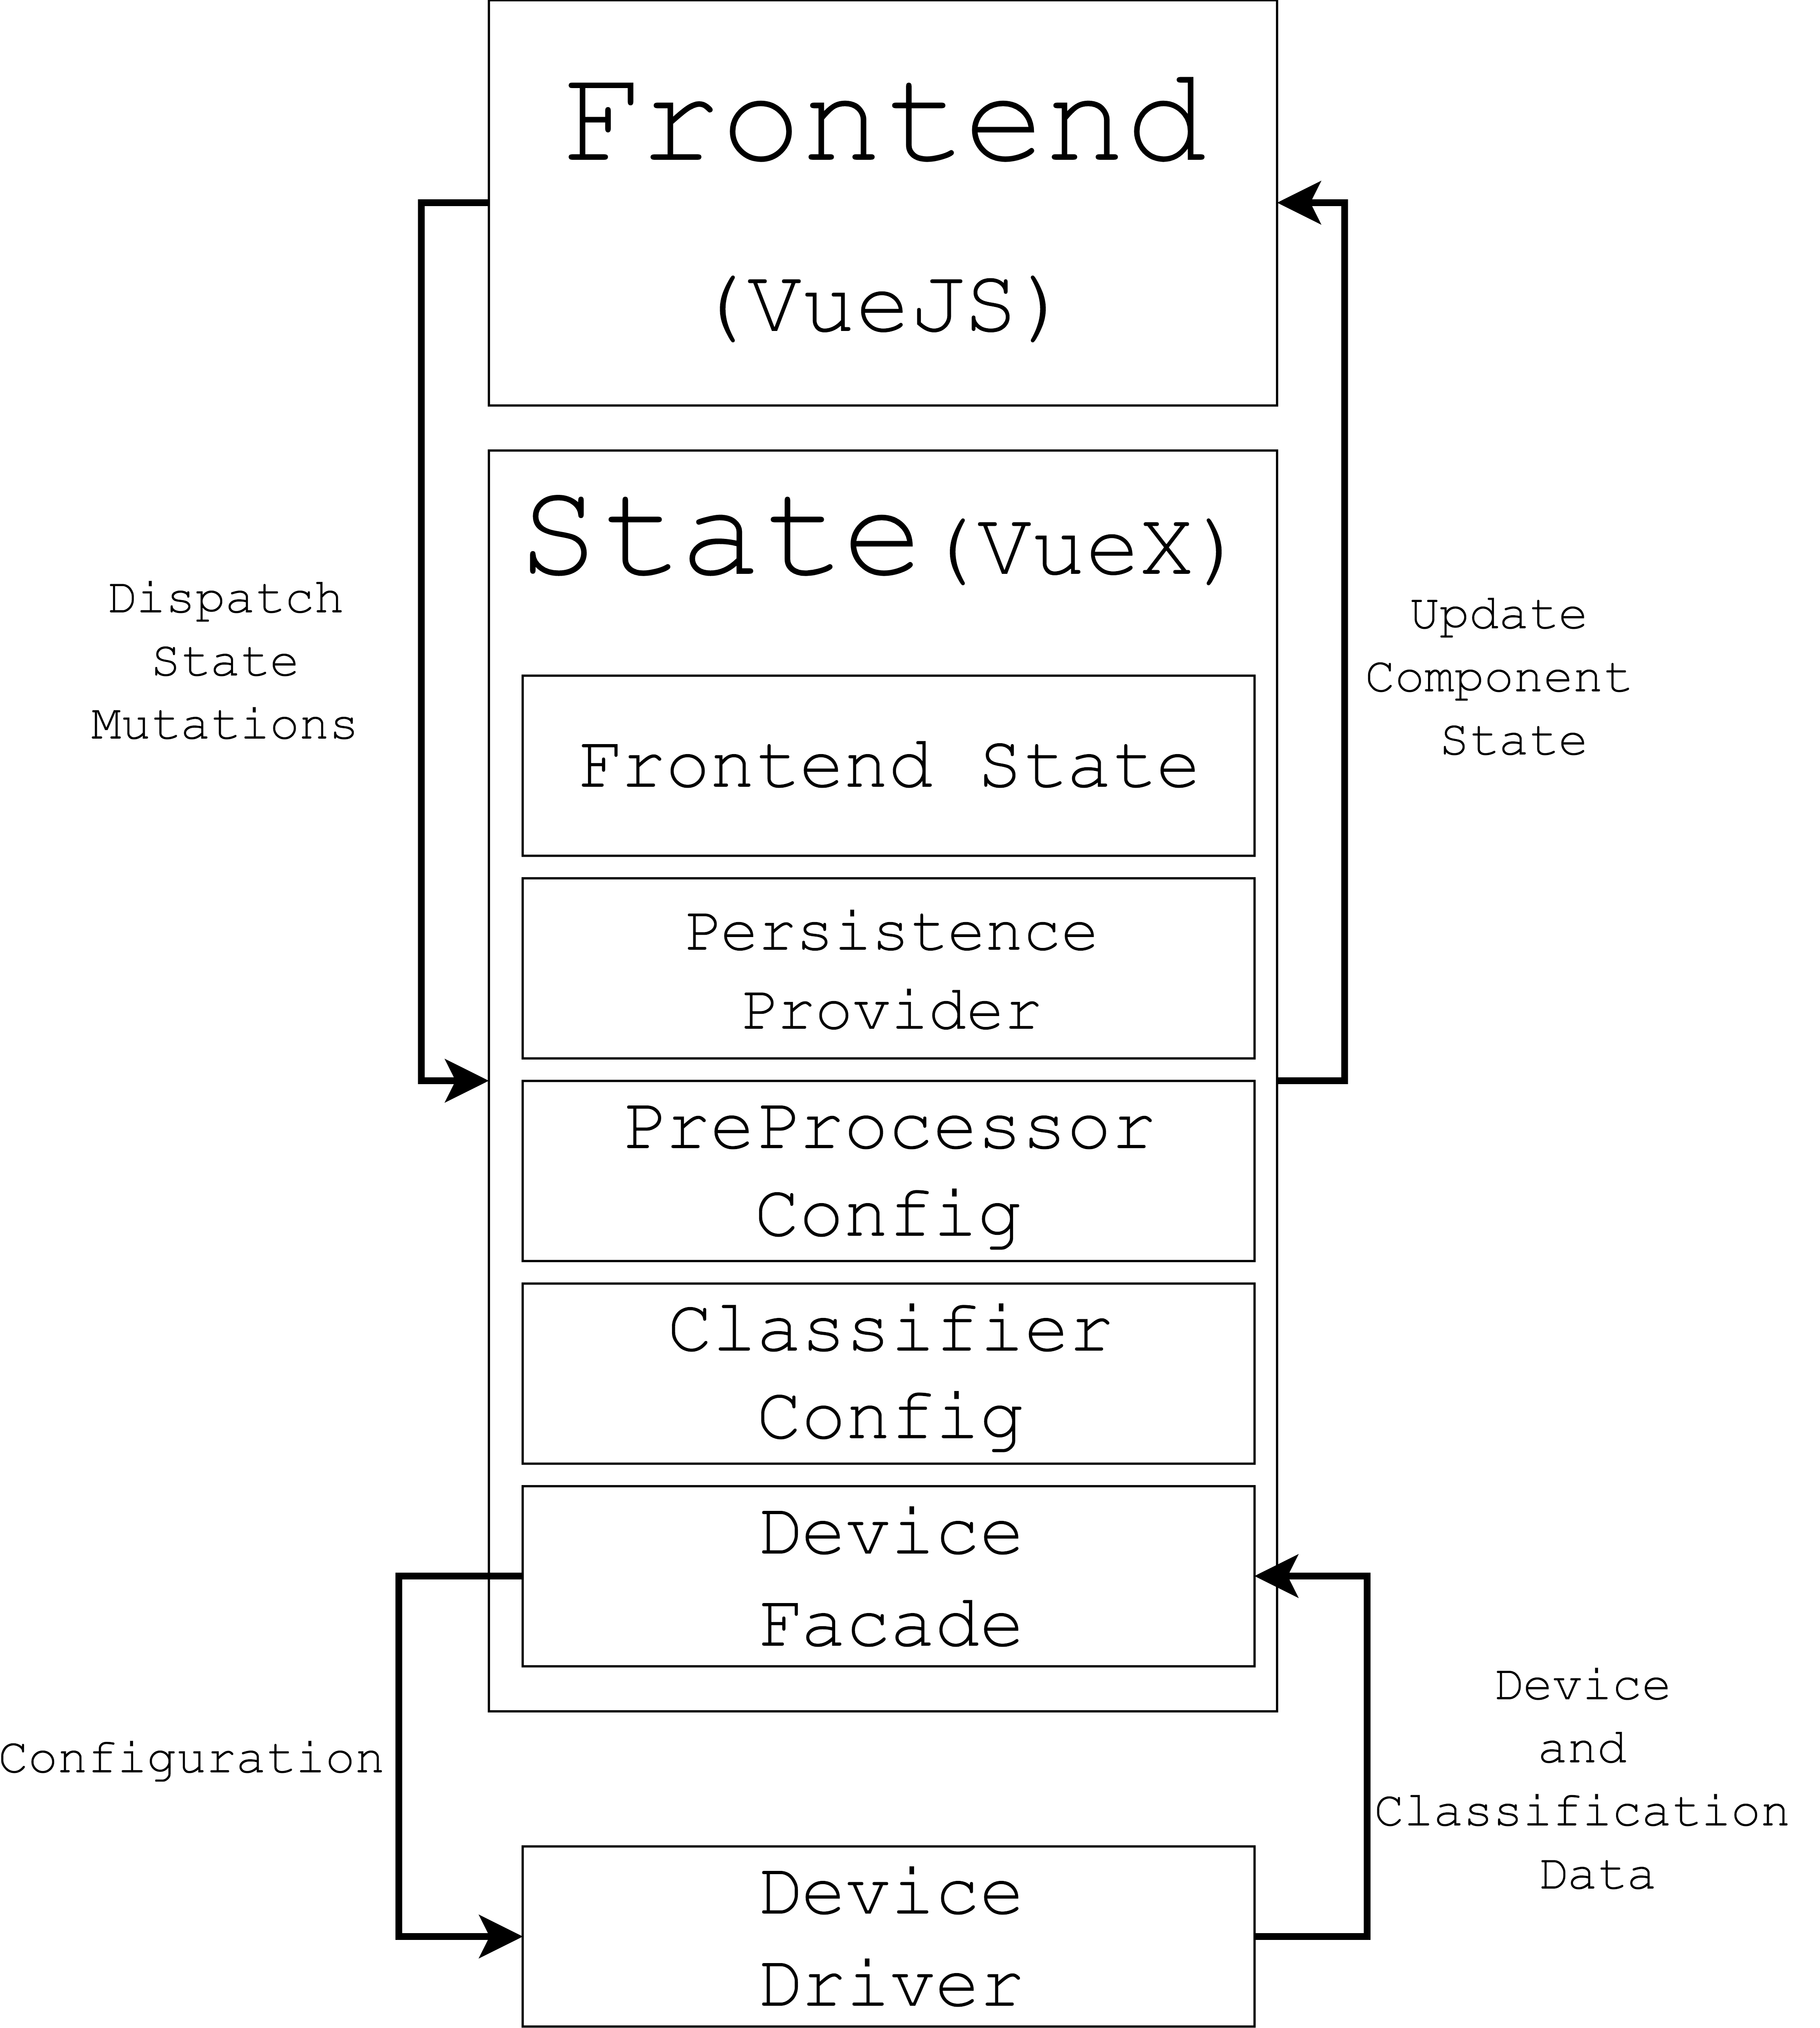
\includegraphics[width=10cm]{highlevelarch}
    \caption{High Level Architecture Overview}
    \label{fig:high-level-architecture}
\end{figure}
A high level overview of the resulting architecture is outlined in Figure \ref{fig:high-level-architecture}. High level architecture components are prepresented as rectangles, relations between them are displayed as arrows. An \emph{includes} relationship is illustrated by nested rectangles. The architecture closely follows the state management pattern recommended by Vuex. 

The Frontend, illustrated by a single rectangle in this case, communicates with the Application State by signifying desired state changes (for example, the ticking of a checkbox) by commiting mutations. At the same time, the Frontend components declare a dependency on relevant parts of the state. If these parts of the state update, Vuex automatically rerenders the dependant Frontend components in order to reflect the changes.

The Application State itself contains, apart from the state of the Frontend Components, references to the other subcomponents of the application, namely references to a component facilitating persistence, configuration information for data preprocessors and classifiers, and finally a reference to the device facade component, which facilitates access to the device driver implementation. These components are further elaborated in the following sections. 

\subsection{Frontend}
\label{sec:impl:frontend}
\begin{figure}[h]
    \centering
    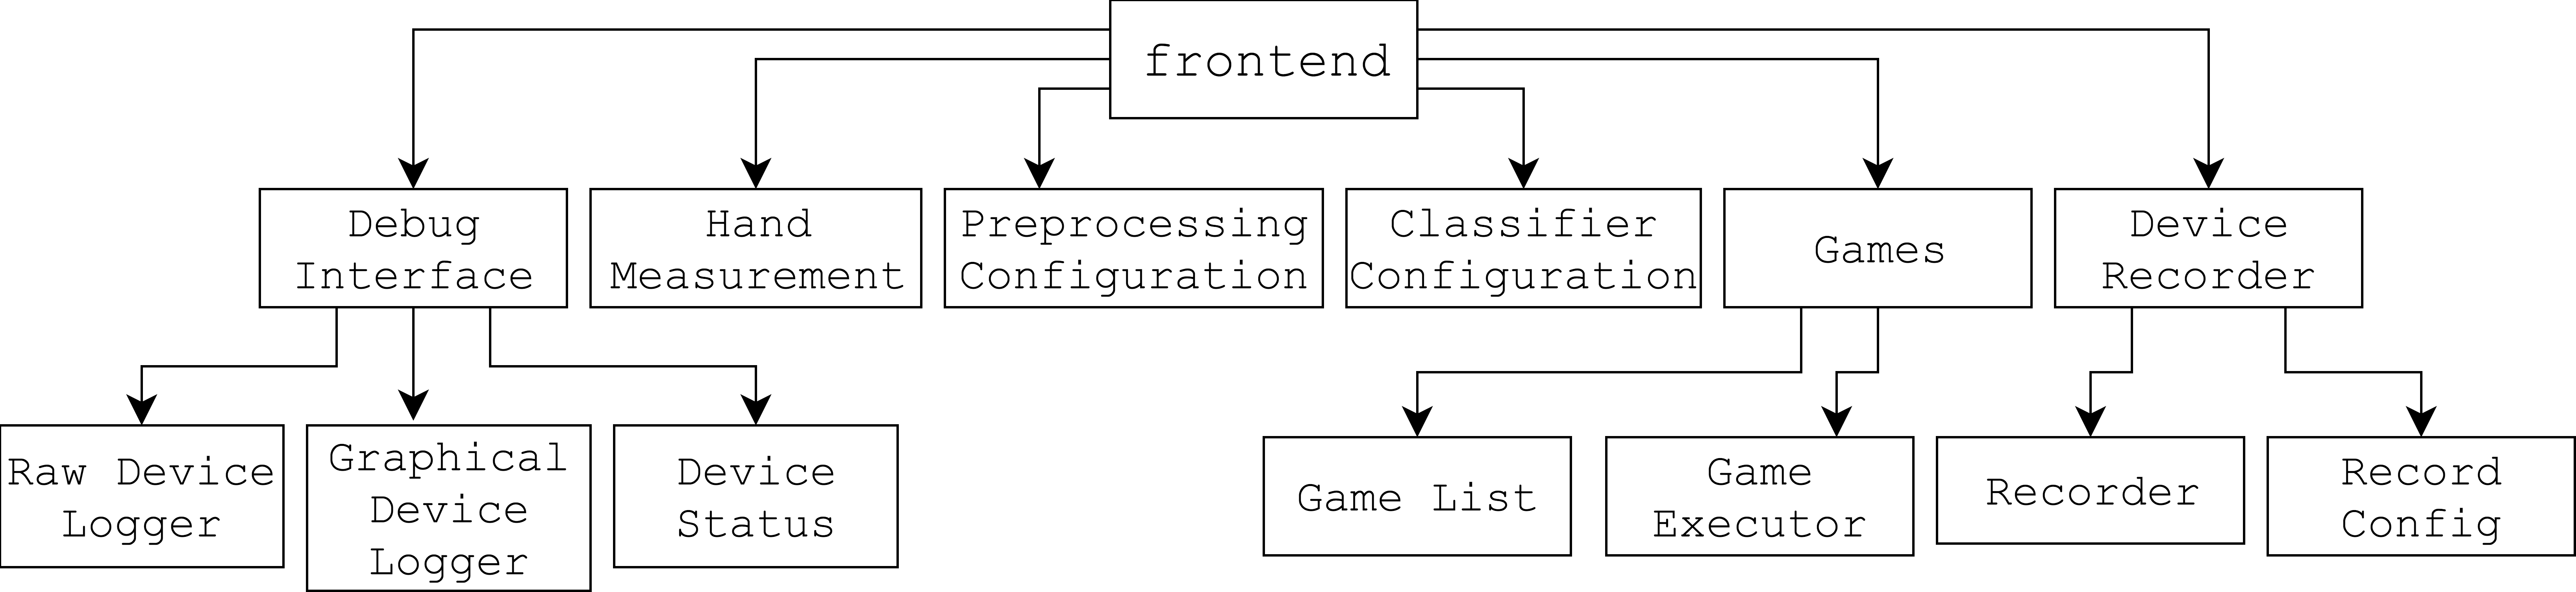
\includegraphics[width=14cm]{frontend}
    \caption{Frontend: Detailed Subcomponent Overview}
    \label{fig:frontend-overview}
\end{figure}

As Figure \ref{fig:frontend-overview} illustrates, the frontend is divided in a number of subcomponents, each responsible for fulfilling a specific purpose.

\subsubsection{Debug Interface}
The Debug Interface is responsible for diagnosing problems if the connection to the motion tracking device cannot be established, and for providing development tooling. It is thus mainly responsible for contributing towards the Extensibility \gls{NFR} (section \ref{sec:nfr:extensibility}). The Interface consists of three subcomponents.

\paragraph*{Raw Device Logger}

The Raw Device Logger is a Frontend Component capable of displaying the raw device frames as they arrive. The component receives the incoming data stream, and formats it in order to be human readable. As new data arrives, the Component updates itself automatically, making it possible to inspect the incoming device data over time. The Component acts as a developer tool, allowing the developer to view live device data, and thus gain intuition over how the device data is structure and how it is changing over time.

\paragraph*{Graphical Device Logger}

Similarly, the Graphical Device Logger is acting on the incoming device data stream, but instead of formatting the raw data in a textual manner, it is interpreted graphically. Using the Three.JS library (\ref{sec:tech:threejs}), graphical hand and finger objects are created and displayed inside a 3-dimensional coordinate system.

\begin{figure}[ht]
    \centering
    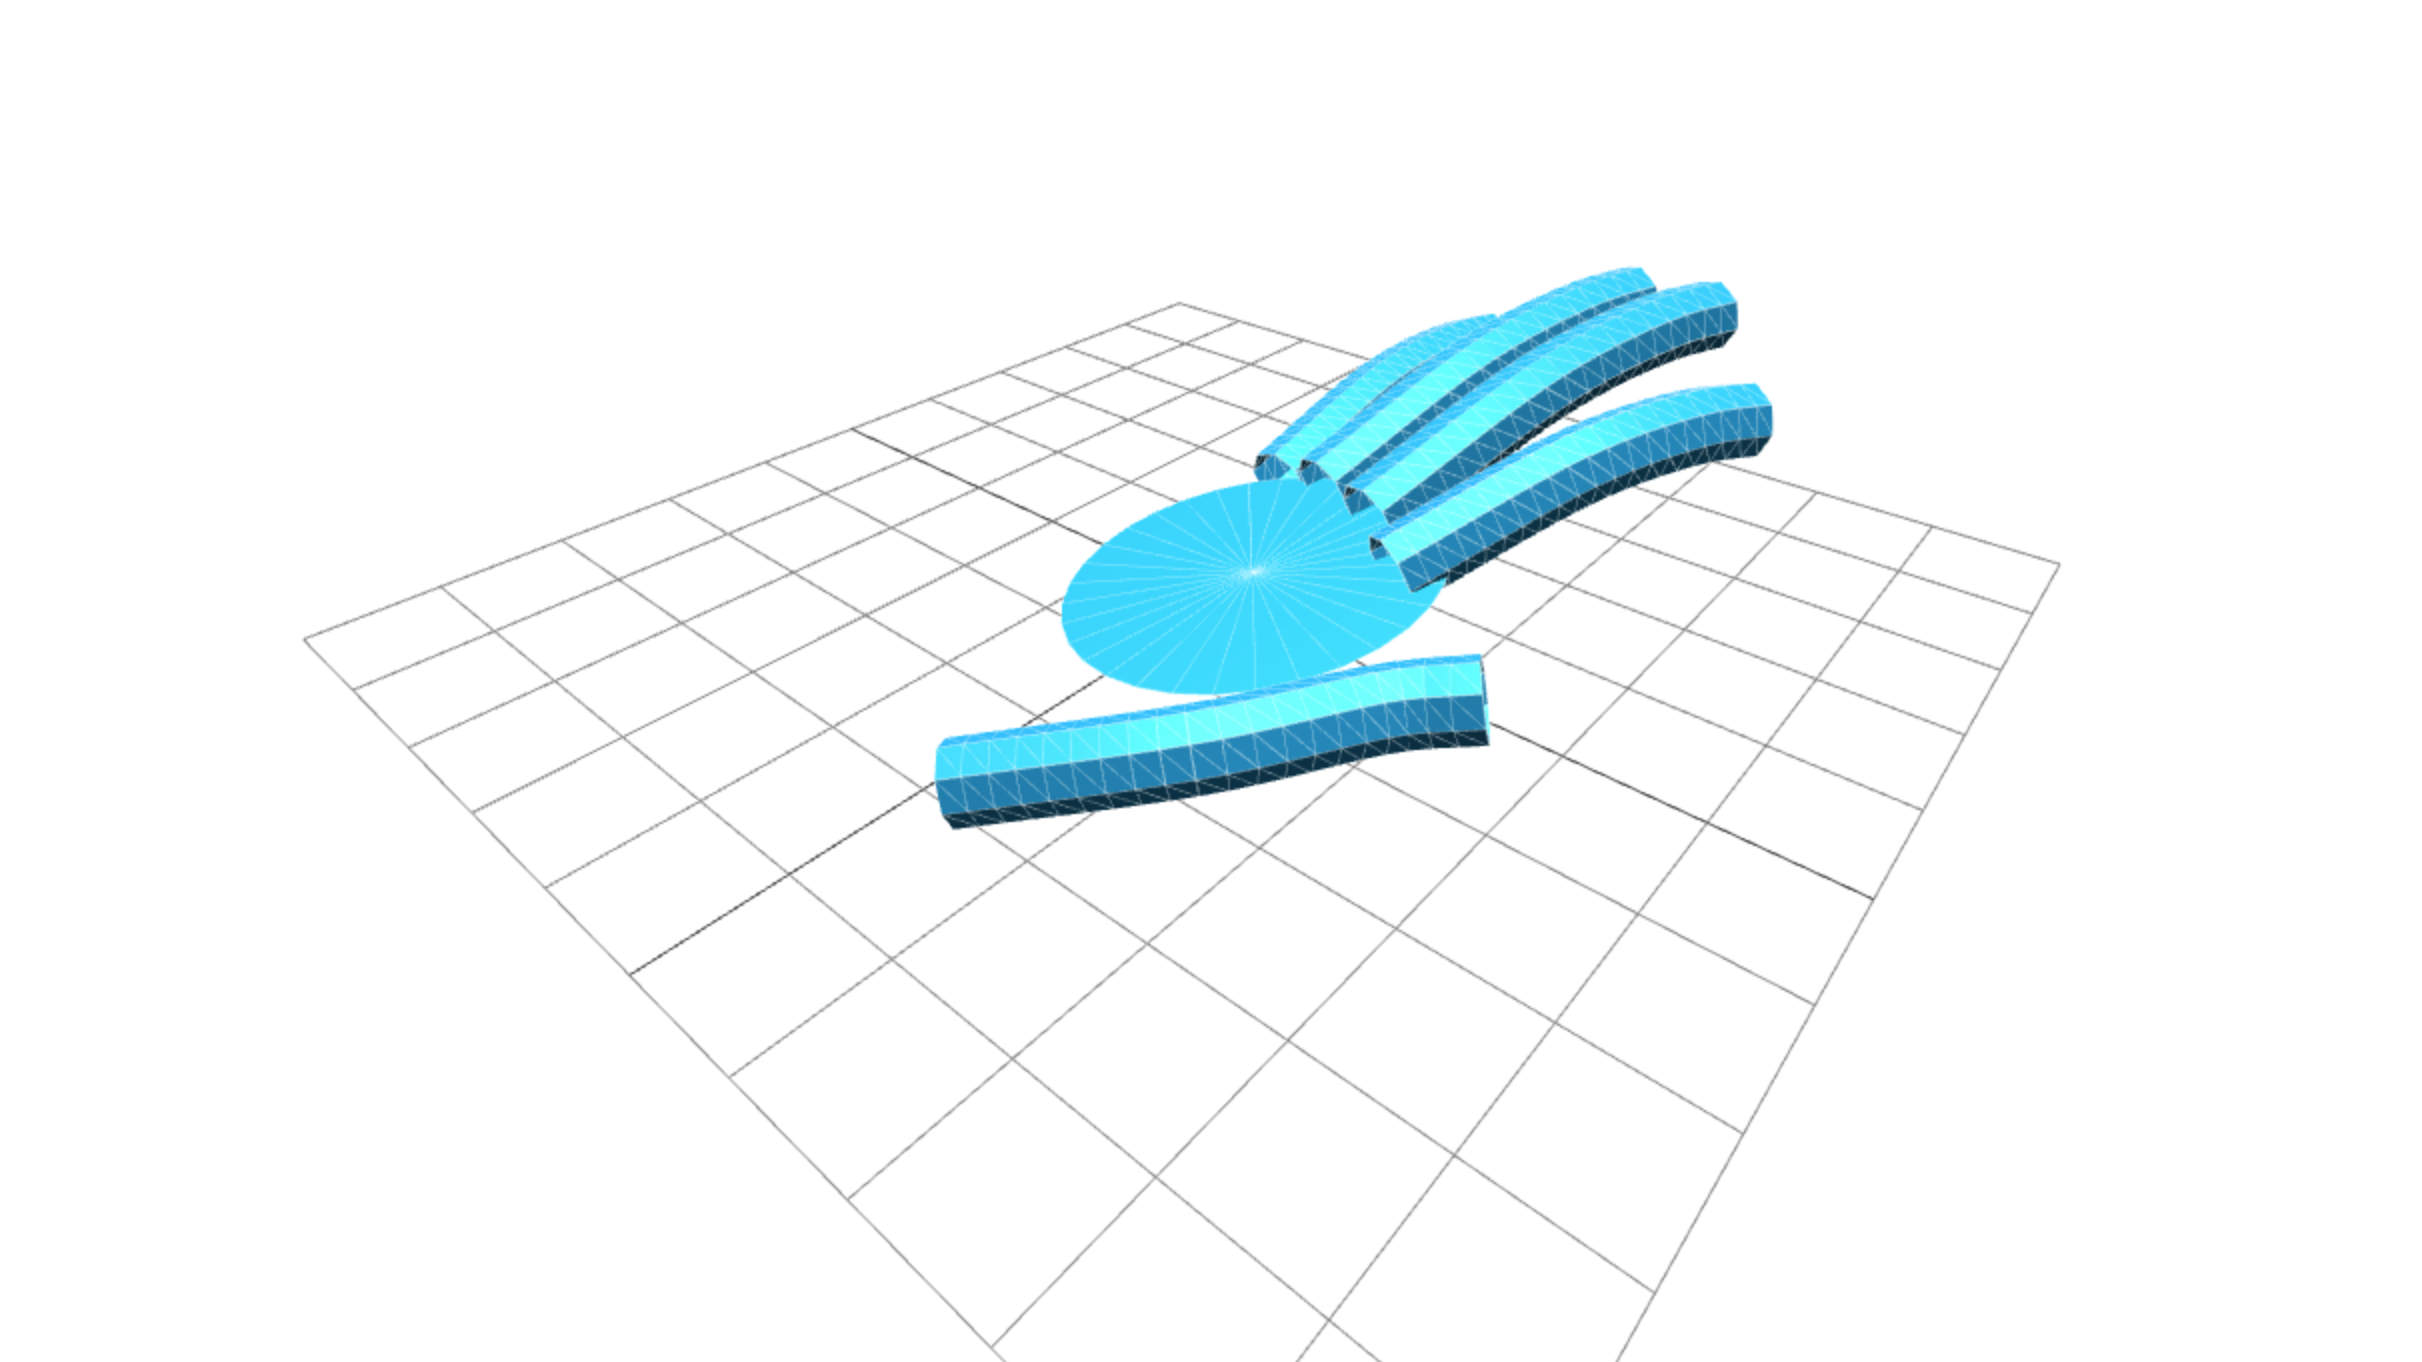
\includegraphics[width=8cm]{graphical-hand-logger}
    \caption{The Graphical Hand Logger.}
    \label{fig:graphical-hand-logger}
\end{figure}

Figure \ref{fig:graphical-hand-logger} illustrates the graphical representation the component is able to produce for Leap Motion Device Data. The Component is able to display other device data as well, though only illustrations based on Leap Motion Device Data are implemented as part of this work. The Leap-Motion specific illustration is constructed by first projecting the interactionBox-relative positional device data (see section \ref{sec:tech:leap-domain-model}) in the THREE.js coordinate system by applying the formula

\begin{equation}
x_{proj} = proj_{min} + (proj_{max} - proj_{min}) * \dfrac{x_{leap} - iBox_{min}}{iBox_{max} - iBox_{min}}    
\end{equation}

to each dimension of relevant positional data, where $x_{proj}$ is the target position, $proj$ describes the bounds of the target projection, $x_{leap}$ is the positional data of the Leap Motion Device, and $iBox$ describes the bounds of the interactionBox. 

Afterwards, the palm is drawn by constructing a 2-dimensional disc, and sizing, positioning, and rotating it according to the transformed hand data. The fingers are drawn by constructing a 3-dimensional tube from each pointable object of the frame data. The tube is constructed from the skeletal tracking information of the pointable and interpolated using a Centripetal Catmull-Rom spline. This type of interpolating curve is widely used in the field of computer graphics because of several useful mathematical properties \cite{Yuksel2011}.

\paragraph*{Device Status Log}
The Device Status Log is the final debugging component of the framework. The Status Log portrays the state of the three main failure points of the application. The main failure points include the connection of the Javascript Device Driver to the Native Device Driver (see \ref{sec:tech:leap-hardware-driver}), the availability of the Native Device Driver, and the Physical availability of the hardware tracking device. The Framework is able to detect the state of all three of these failure conditions, and displays instructions to the user on how to mitigate these problems in case one or more failures occur.

\subsubsection{Hand Measurement}
The ergo therapist is required to measure angles between certain bones of the hand in order to determine how the patient is progressing in recovery \cite[sec. 4.1.6]{StudiArbeitVolzBaumotte}. The digitized ergo therapy system should be able to perform these measurements as well in order to reduce the manual workload of the therapist.

The reference implementation of the system includes a frontend component with the ability to take measurements of the angles between neighboring fingers. Other types of measurements are able to be integrated in the framework easily by using existing code structure and utility functions. The measurements are able to be averaged across a configurable timeframe in order to achieve more accurate results. The angle calculation itself is performed by applying the formula

%export const calculatePointableAngle = (
%  first: LeapPointable,
%  second: LeapPointable
%): number => {
%  const ab = first.direction
%    .map((el, idx) => el * second.direction[idx])
%    .reduce((p, c) => p + c, 0);
%  const normFirst = norm(first.direction);
%  const normSecond = norm(second.direction);
%  const theta = Math.acos(ab / (normFirst * normSecond));
%  return theta * 180 / Math.PI;
%};
\begin{equation}
angle = \arccos(\dfrac{\vec{p_1} * \vec{p_2}}{\norm{\vec{p_1}} * \norm{\vec{p_2}}}) * \dfrac{180}{\pi}
\end{equation}

to the directional vectors of neighboring fingers.

\subsubsection{Preprocessing and Classification Configuration}
The stream pre-processing and classification frameworks, outlined in further detail in sections \ref{sec:impl:preprocessing} and \ref{sec:impl:classify} respectively, require user configuration from the frontend. The available subcomponents that are available for each framework can be toggled on or off, and supplied with configuration that the subcomponent requires. Every change made in the Frontend configuration will automatically be propagated through the system, and will be available immediately.

\subsubsection{Game Listing}
The most integral part of the system is for the patient to be able to play games by means of performing the relevant recovery exercises as dictated by the therapist (see section \ref{sec:frs}). In order to implement this functionality in the system, the frontend has a component where the available Games are listed. For each available Game, a short title and description is shown. Furthermore, this component validates if the system is ready to execute the game (i.e., the motion tracking device is plugged in and functioning normally, and a classifier has been activated, as outlined in \ref{sec:impl:classify}). After the component has validated that the system is ready, a Play Button becomes available to the user. After the Play Button has been pressed, the component hands control to the Game Execution Framework (see section \ref{sec:impl:gameexec}).

\subsubsection{Hand Recorder}
The Hand Recorder is a Frontend Component with the primary purpose to alleviate framework developers from having to physically connect a hand tracking device in order to develop preprocessors, classifiers, or games for the platform. The component allows to record series of device frames. Optionally, the recordings may be titled, and persisted in the Persistence Provider implementation (see section \ref{sec:impl:persist}). If a previously saved recording is activated using this component, the contained frames will be propagated in an endless loop through the framework as if they were coming from a physical device. Only one saved recording may be active at any given time. If a hand tracking device is already connected and functioning as expected, the data coming from the recording will be preferred. Furthermore, the user is able to download saved recordings, for example in order to reproduce bugs, or using them for illustration purposes in other parts of the system.

\subsection{Device Facade Interface}
The Device Facade Interface is the primary access point for frontend components that wish to work with motion tracking device data. The Interface, named after the well-known Facade pattern in Software Development \cite{Gamma:1995:DPE:186897}, decouples the Frontend Components both from the actual implementation of the Device Driver (see section \ref{sec:impl:driver}), as well as the actual data source (i.e., Recording, Physical, or potential future data sources).


Figure \ref{fig:device-facade-interface} shows an excerpt of the Interface. References to \gls{RX} streams representing Hand Tracking Data, Classification Data (see \ref{sec:impl:classify}), and the DeviceDriver implementation itself may be optained. Additionally, the Facade may receive Configuration updates regarding the Data Preprocessing and Classification Frameworks from Frontend Components, which will subsequently be relayed into the Device Driver for further processing.
\begin{figure}
\begin{minted}{typescript}
export interface DeviceFacade {
    getHandTrackingData: (
      store: Store<RootState>
    ) => Observable<GenericHandTrackingData> | undefined;
    getClassificationStream: () => Observable<ClassificationData> | undefined;
    getDeviceDriver: () => DeviceDriver;
    updatePreProcessors: (x: PreProcessorConfig[]) => void;
    updateClassifier: (x: ClassifierConfig) => void;
    ...
}
\end{minted}
\caption{Device Facade Interface Definition (excerpt)}
\label{fig:device-facade-interface}
\end{figure}
The Interface is bound to the desired Implementation at compile time through dependency injection, and registered to the global application state on page load.

The System contains a reference implementation of the Device Facade Interface, named \emph{AllPurposeFacade}, though different implementations, for example a mock implementation for utilization in Unit Tests, are conceivable.
\subsection{Device Driver Interface}
\label{sec:impl:driver}
Components implementing the Device Driver Interface are primarily responsible for handling the connection to the physical device from the Web Context. In case of the Leap Motion Platform, such a connection is obtained by connecting to a local Websocket Server provided by the Leap Motion Hardware Device Driver \emph{leapd} (see section \ref{sec:tech:leap-hardware-driver}). Other potential Motion Tracking Devices, such as the Microsoft Kinect Platform, provide similar methods of accessing the Hardware Device from a Web Context \cite{KinectSDK}. New Device support can thus be added to the platform by means of adding a Device Driver Implementation, and optionally providing the parts of the Platform that depend on specific Device Data with the relevant device-specific implementations, for example providing rendering methods for the new Device to the Graphical Device Logger (see \ref{sec:impl:frontend}, par. \emph{Graphical Device Logger}).
\begin{figure}
\begin{minted}{typescript}
export interface DeviceDriver {
  deviceName: string;
  establishConnection: () => Observable<DeviceConnectionState>;
  getTrackingData: () => Observable<GenericHandTrackingData>;
  getClassificationData: () => Observable<ClassificationData> | undefined;
  enableClassification: (classifiers: string[]) => void;
  updatePreProcessors: (configs: PreProcessorConfig[]) => boolean;
  updateClassifier: (config: ClassifierConfig) => boolean;
  digest: (data: GenericHandTrackingData) => void;
  ...
}
\end{minted}
\caption{Device Driver Interface Definition (excerpt)}
\label{fig:device-driver-interface}
\end{figure}

Figure \ref{fig:device-driver-interface} illustrates the methods and properties that must be implemented by Device Drivers. The \texttt{deviceName} property must be defined on the implementing class. This property acts as a unique device identifier across the whole system. If device specific implementations are required for some parts of the system, they are resolved using this identifier. The method \texttt{establishConnection} is used to signal to the DeviceDriver that a connection should be established. This method is called on system start. The method must return a \gls{RX} Observable representing the connection state to the device driver over time. After \texttt{establishConnection} has been called, the DeviceDriver should automatically attempt to reconnect to the native device driver if the connection has been lost or could not be established initially, and update the Observable on each registered change of connectivity.

The \texttt{getTrackingData} method must return a \gls{RX} Observable that should emit the tracking data each time a new frame is received by the driver. The generic type of a device frame is named \texttt{GenericHandTrackingData}. The concrete implementations of the Interface may extend this type in order to explicitly type the data coming from the device. The methods \texttt{enableClassification}, \texttt{updatePreProcessors}, and \texttt{updateClassifier} are used to signal to the device driver that its internal Data Preprocessing and Classification pipelines should update. These subcomponents of the Device Driver are further explained in sections \ref{sec:impl:preprocessing} and \ref{sec:impl:classify}.

\subsection{Persistence Framework}
\label{sec:impl:persist}
\subsection{Stream pre-processing framework}
\label{sec:impl:preprocessing}
\subsection{Classification framework}
\label{sec:impl:classify}
\subsection{Game Execution Framework}
\label{sec:impl:gameexec}




\section{Development Pipeline}
Webpack 4

VueJS 2, Vue Router, VueX, inversify Dependency Injection

Karma Unit Tests

THREE.js
\section{Implemented Subsystems}
\subsection{Device Driver Interface}
Describe Generalized Device Driver Interface. Point out that adding different devices is possible with this architecture.
\subsection{Device Facade}
Justify for a need of a Facade in Front of the raw Device Driver: Seperation of Concerns and Recording (Mock data) Functionality. Ease of Testing.
\subsection{Device Debug Interface}
Describe Component: Raw Device Logger, Device Status Log, Device Graphical Log
\subsection{Graphical Hand Logger}
THREE.JS, OrbitControls, Smoothing, Prop Configuration
\subsection{Device Recorder}
Record Segments of hand movements in order to aid in development, make classification errors reproducible
\subsection{Persistence Provider}
Describe Abstract Persistence Provider Interface

Describe Concrete Persistence Provider Interface Implementation: IndexedDB
\subsection{Preprocessing Framework}
Justify need for Preprocessing: Lots of useless data coming from the device. Preliminary
clean up of data may be relevant for all classifiers
\subsection{Classification Framework}
Describe how Classifiers receive the preprocessed data frame stream, and transform the stream in order to emit another stream of classifications, along with relevant metadata
\subsection{Game Execution Engine}
Describe how Games are receiving the Classification Stream and using that in order to drive the gameplay.

